\section{Risultati}
\subsection{Obiettivo 1}
\begin{frame}{\subsecname}
    
    \begin{columns}
        \begin{column}{.63\textwidth}
            Scenario con carico \(\lambda = 6.66\) req/s: analisi del tempo di risposta medio in funzione della soglia \(SI_{max}\).
            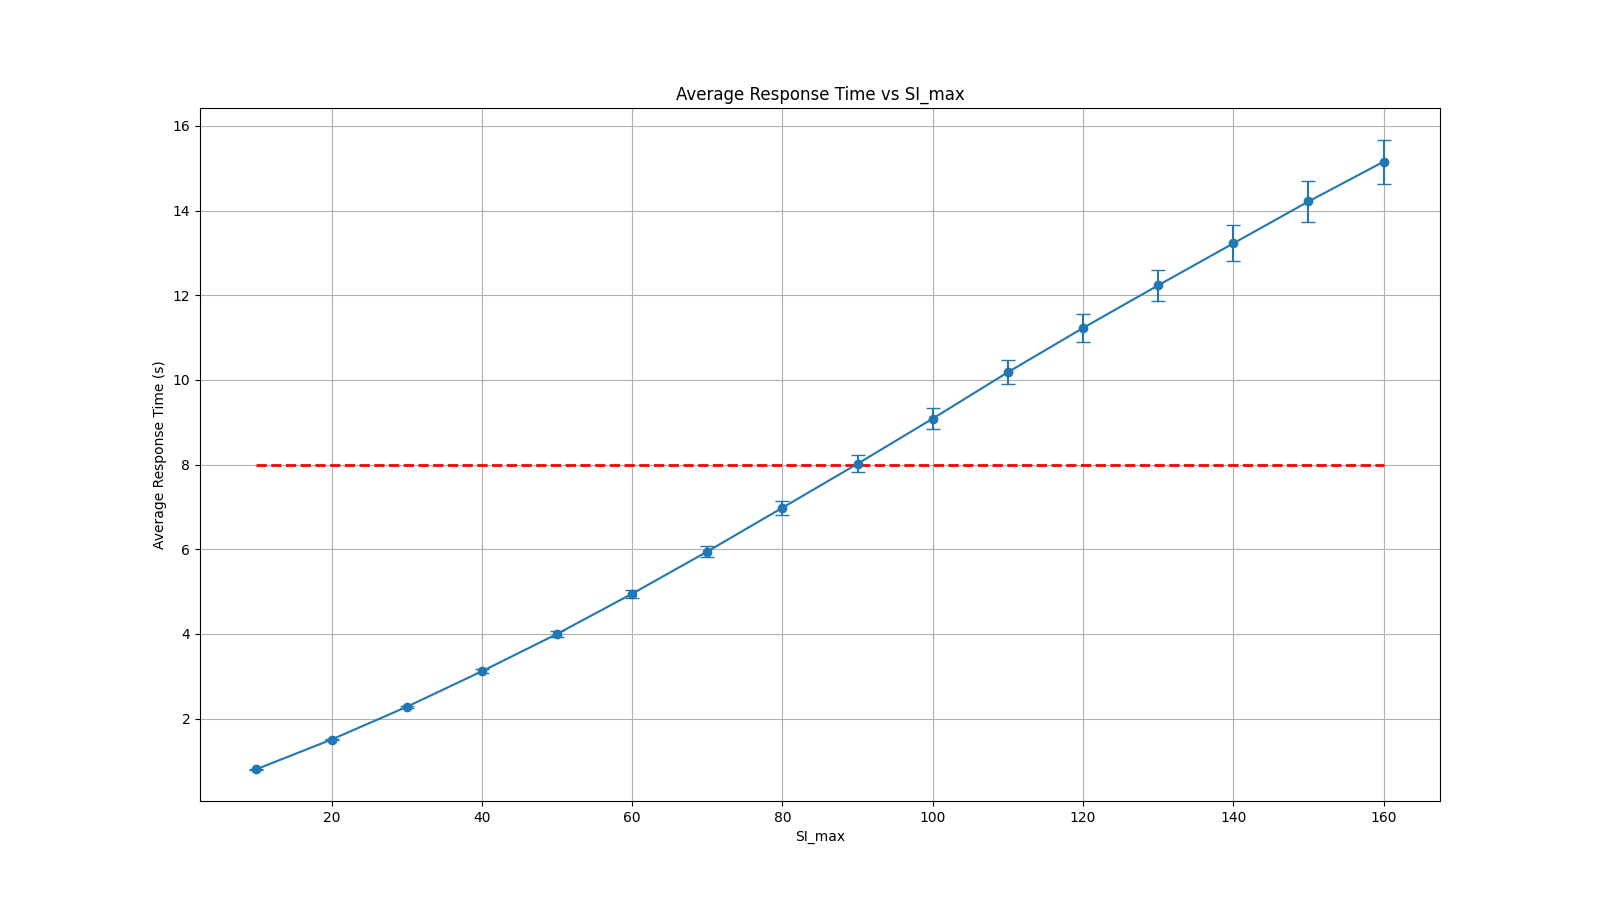
\includegraphics[trim={3.5cm 1cm 4cm 2cm}, clip, width=1\textwidth]{../images/response_time_vs_si_max.png}       
            
        \end{column}
        \begin{column}{.32\textwidth}
            \begin{block}{}
                \begin{itemize}
                    \item Il tempo di risposta cresce all'aumentare di \(SI_{max}\)
                    \item \( SI_{max} = 90 \) è a rischio
                    \item \( SI_{max} = 80 \), massimizza l'uso del webserver mantenendo \( E[R] < 8s \)
                \end{itemize}
            \end{block}
        \end{column}
    \end{columns}
\end{frame}

\subsection{Obiettivo 2}
\begin{frame}{\subsecname}
     \begin{columns}
        \begin{column}{.32\textwidth}
            \begin{block}{}
                \begin{itemize}
                    \item Fino a \(\lambda = 7\) req/s 
                    \begin{itemize}
                        \item \(E[R]\ \nearrow\) 
                        \item \(SI <SI_{max}\)
                    \end{itemize}
                    \item da \(\lambda = 8\) req/s 
                    \begin{itemize}
                        \item Spike server in azione
                        \item \(E[R]\ \searrow\) 
                    \end{itemize}
                    \item da \(\lambda = 11\) req/s 
                    \begin{itemize}
                        \item Saturazione spike server
                        \item \(E[R]\ \nearrow\)
                    \end{itemize}
                \end{itemize}
            \end{block}
        \end{column}
        \begin{column}{.63\textwidth}
            Scenario con vari scenari di soglia: analisi del tempo di risposta medio in funzione di \(\lambda = {1, 2, ..., 12}\) req/s.
            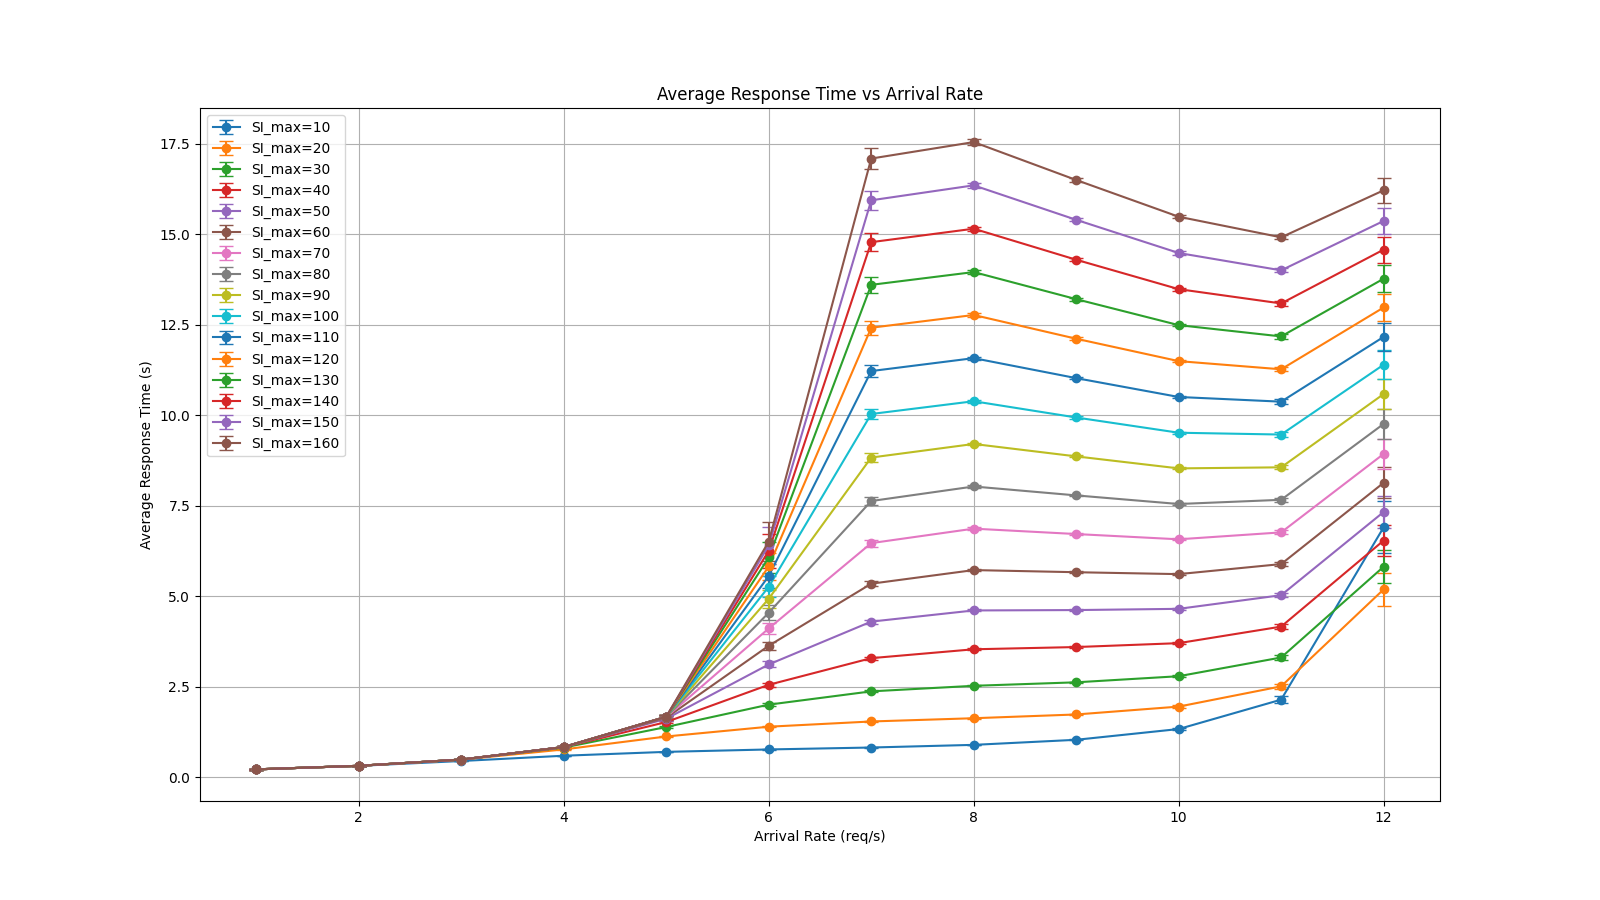
\includegraphics[trim={3.5cm 1cm 4cm 2cm}, clip, width=1\textwidth]{../images/response_time_vs_arrival_rate_vs_si_max.png}            
        \end{column}
        
    \end{columns}
\end{frame}

\subsection{Obiettivo 3}
\begin{frame}{\subsecname}
    \begin{columns}
        \begin{column}{.63\textwidth}
            Spike server potenziato del doppio (\(E[S] = 0.08s\)): analisi del tempo di risposta medio in funzione di \(\lambda = {1, 2, ..., 12}\) req/s.
            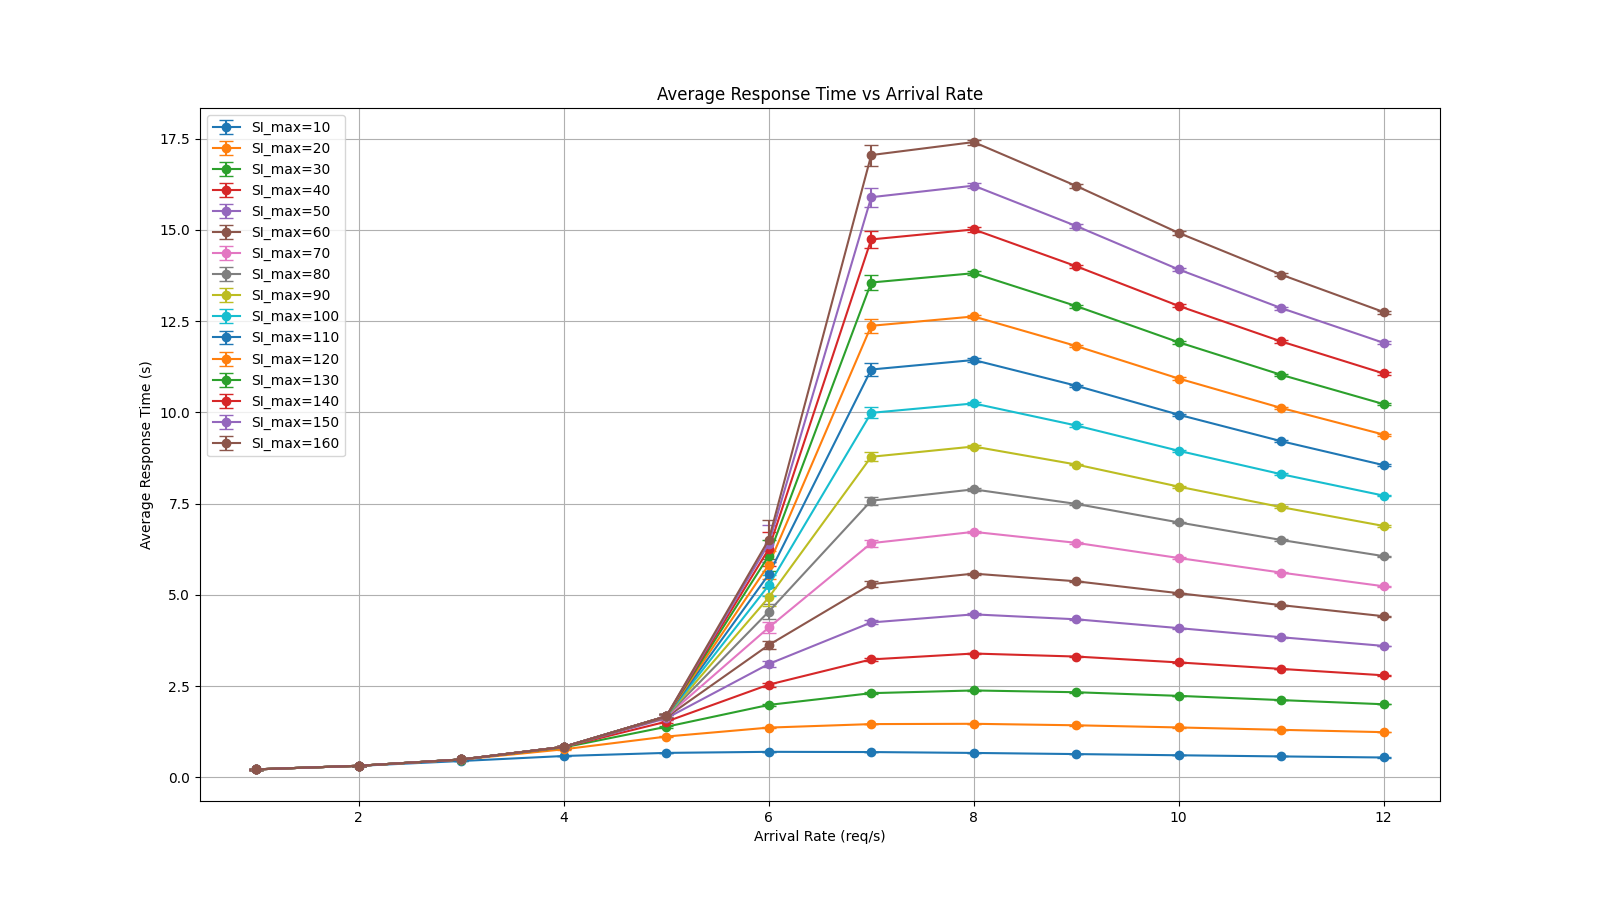
\includegraphics[trim={3.5cm 1cm 4cm 2cm}, clip, width=1\textwidth]{../images/response_time_vs_arrival_rate_vs_si_max_enhanced_spike.png}            
        \end{column}
        \begin{column}{.32\textwidth}
            \begin{block}{}
                \begin{itemize}
                    \item Comportamento equivalente all'obiettivo 2
                    \item Spike server non si satura più
                \end{itemize}
            \end{block}
        \end{column}
        
        
    \end{columns}
\end{frame}